\section{Problemas polinomiais não determinísticos}
Problemas polinomiais não determinísticos ou apenas problemas \textbf{NP} é uma classe de problemas que não se conseguiu até este momento criar algoritmos determinísticos que os resolvam em tempo satisfatório \cite{goodrichprojeto}. 

Para esse tipo de problemas utiliza-se algoritmos não determinísticos como parte da solução e cria-se mecanismos para fazer a validação da solução "encontrada". Essa validação deve ter custo polinomial para que faça sentido o uso desta abordagem. 

Podemos definir de forma mais informal que algoritmos não determinísticos são algoritmos que basicamente "escolhem" uma solução entre todas as possíveis soluções, sem nenhum critério de escolha. Essa "escolha" por sua vez tem custo $O\,(1)$ uma vez que não é realizado nenhum esforço computacional.

Pode-se acrescentar também que todos os problemas em \textbf{P} também estão em \textbf{NP}, ou seja o conjunto de problemas \textbf{P} está contido em \textbf{NP}, isso se dá pelo fato de que podemos resolver qualquer problema \textbf{P} em tempo polinomial \cite{leisersonalgoritmos}.

\begin{figure}[H]
	\centering
	\label{fig1}
	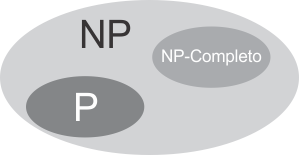
\includegraphics[scale=2]{./figuras/figProblemas.png}
	\caption{$P \neq NP$ \cite{VIEIRA2001}}
\end{figure}
